\subsection{Number of Hops per Route}

We want to look at traceroute measurements. The first thing we analyze is the
average number of hops per traceroute measurement. For that, we use the RIPE
Atlas built-in traceroute measurements. Figure~\ref{fig:hops-per-measument}
shows the histogram of hops for Canada, the United~Kingdom, France, and
Germany. The countries were chosen due to the completeness of the data. Similar
results were found when looking at other countries.

\begin{figure}
	\centering
	\begin{subfigure}[b]{0.48\linewidth}
		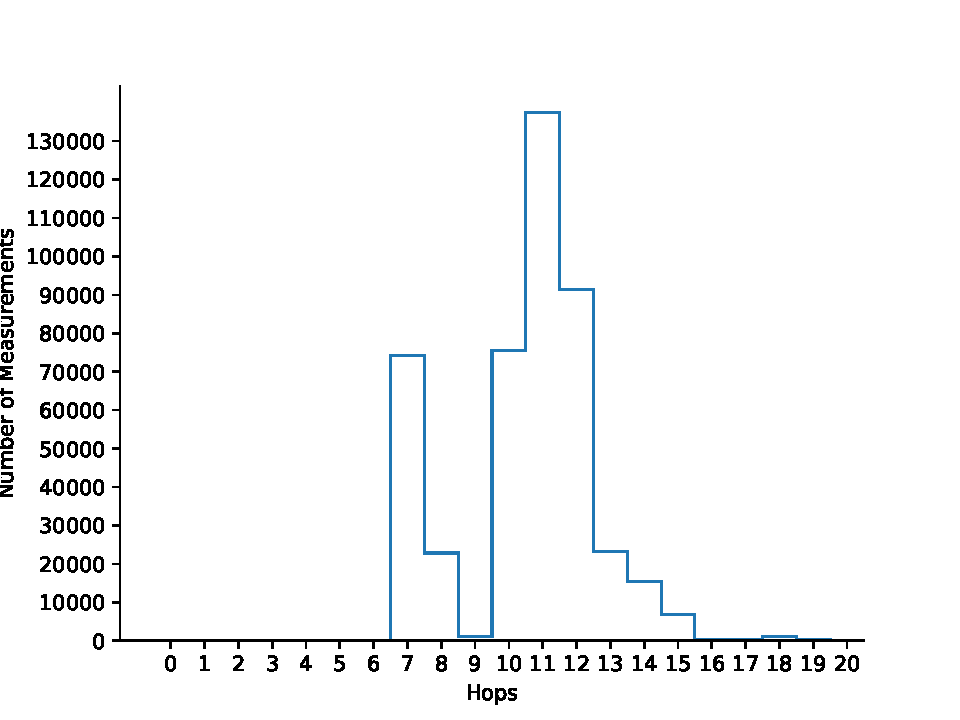
\includegraphics[width=\linewidth]{chapters/4-results/traceroute/img/hops_CA.pdf}
		\caption{Canada}
	\end{subfigure}
	\begin{subfigure}[b]{0.48\linewidth}
		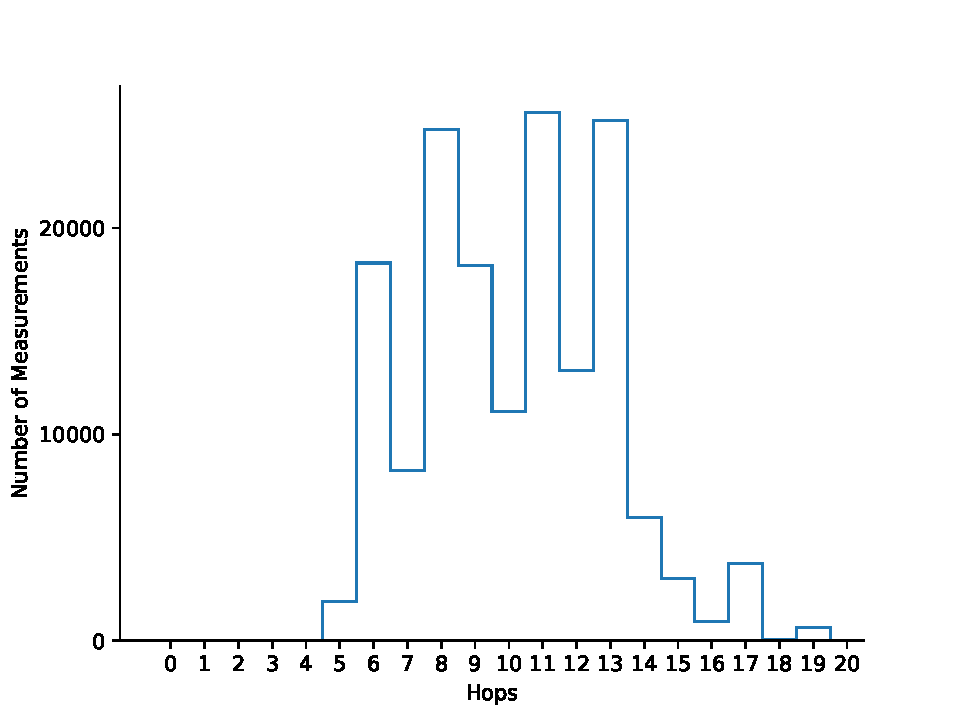
\includegraphics[width=\linewidth]{chapters/4-results/traceroute/img/hops_PH.pdf}
		\caption{Philippines}
	\end{subfigure}
	\begin{subfigure}[b]{0.48\linewidth}
		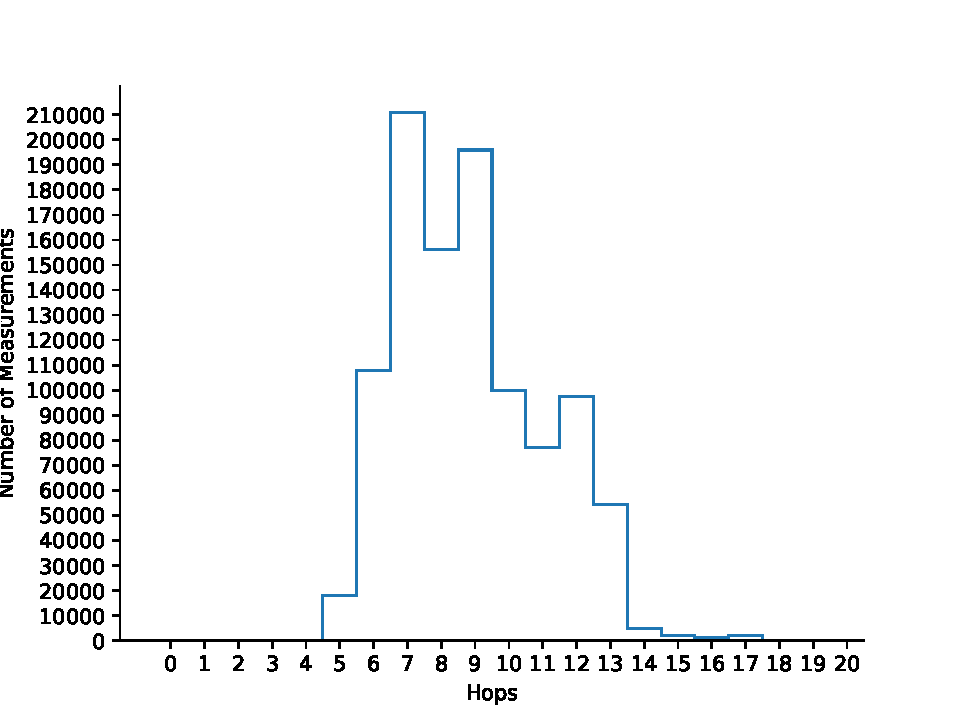
\includegraphics[width=\linewidth]{chapters/4-results/traceroute/img/hops_FR.pdf}
		\caption{France}
	\end{subfigure}
	\begin{subfigure}[b]{0.48\linewidth}
		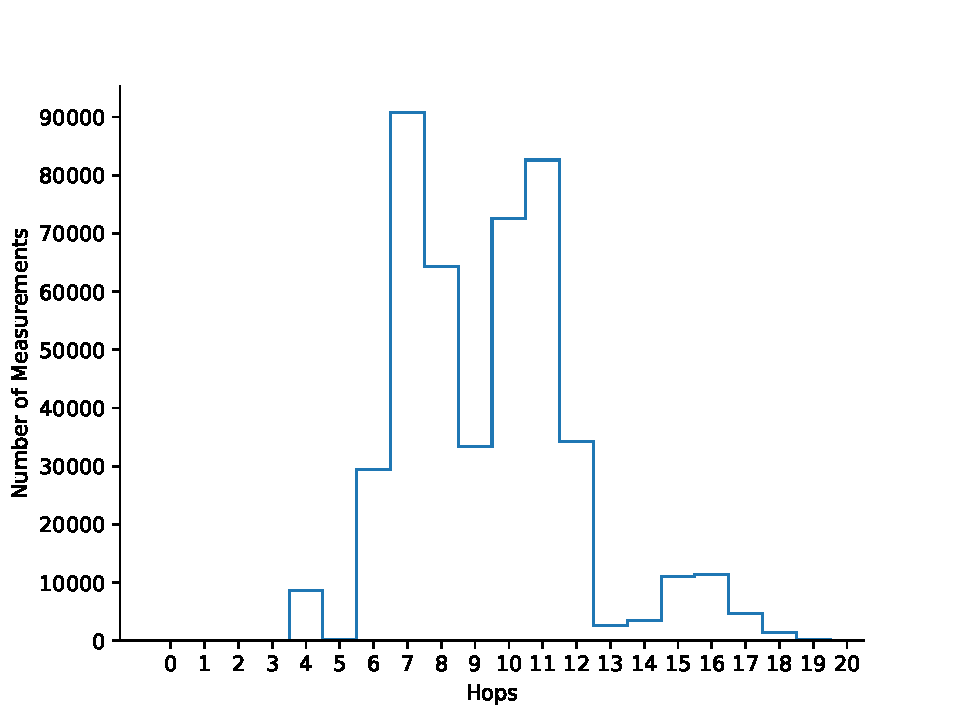
\includegraphics[width=\linewidth]{chapters/4-results/traceroute/img/hops_DE.pdf}
		\caption{Germany}
	\end{subfigure}
	\caption{Histogram of Hops the Traceroute Measurement took.}
	\label{fig:hops-per-measument}
\end{figure}

The histograms show that most routes take between seven and fourteen hops.
It is interesting to note that the histograms show a similar pattern compared
to the histogram for TLS handshake latencies that are shown in
Chapter~\ref{sec:latency-wholerange}. Both histograms have a pattern that
spikes at two points. We assume that there a specific reason for this
correlation that is part of the Starlink network.

\subsection{Latency per Hop}

We want to a closer look on how Starlink latency behaves in each hop. To do so,
we looked at each hop of the built-in measurements of RIPE~Atlas and the change
in round trip time from hop to hop. Figure~\ref{fig:latency-change-per-hop}
show how the round trip time measured in the traceroute measurement behaves
with more hops. It is important to note that in rare cases the RTT does not
increase with more hops, as traceroute measurements work with repetitive
measurements that might yield inconsistent results in consecutive runs.

\begin{figure}
	\centering
	\begin{subfigure}[b]{0.48\linewidth}
		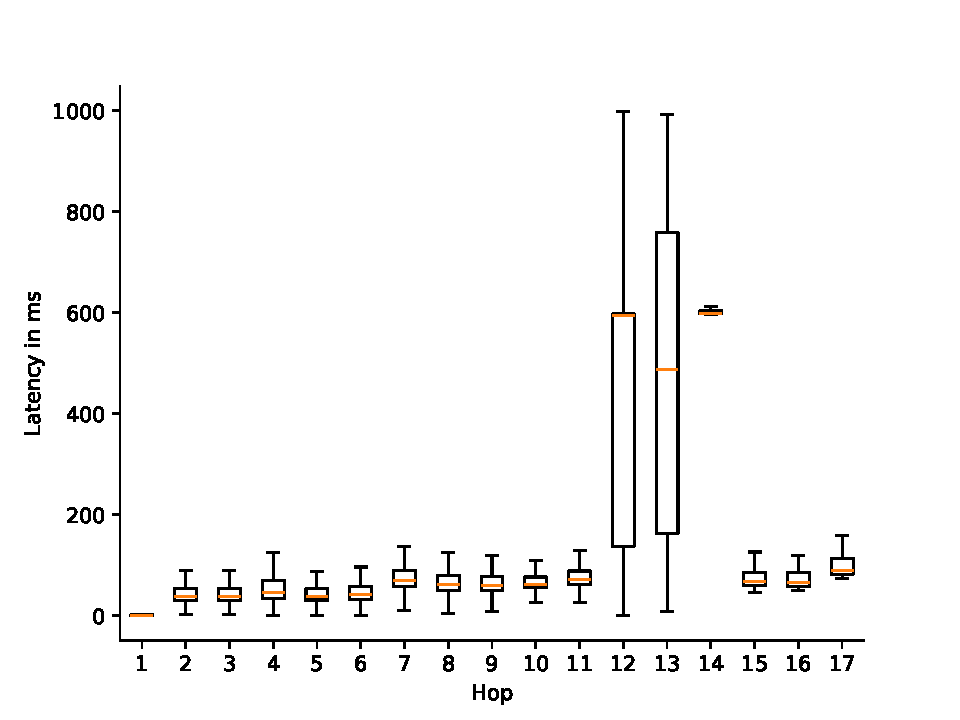
\includegraphics[width=\linewidth]{chapters/4-results/traceroute/img/latency-per-hop-CA.pdf}
		\caption{Canada}
	\end{subfigure}
	\begin{subfigure}[b]{0.48\linewidth}
		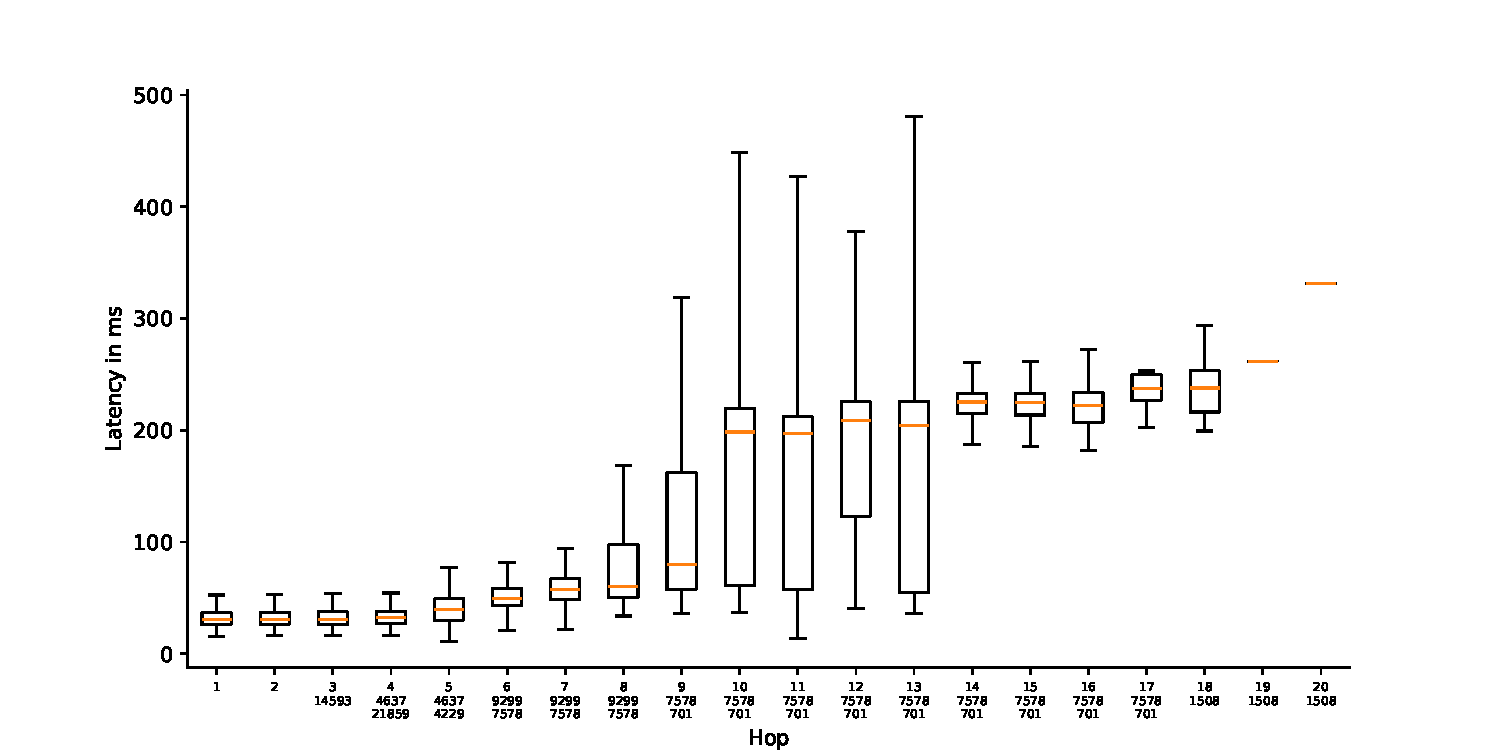
\includegraphics[width=\linewidth]{chapters/4-results/traceroute/img/latency-per-hop-PH.pdf}
		\caption{Philippines}
	\end{subfigure}
	\begin{subfigure}[b]{0.48\linewidth}
		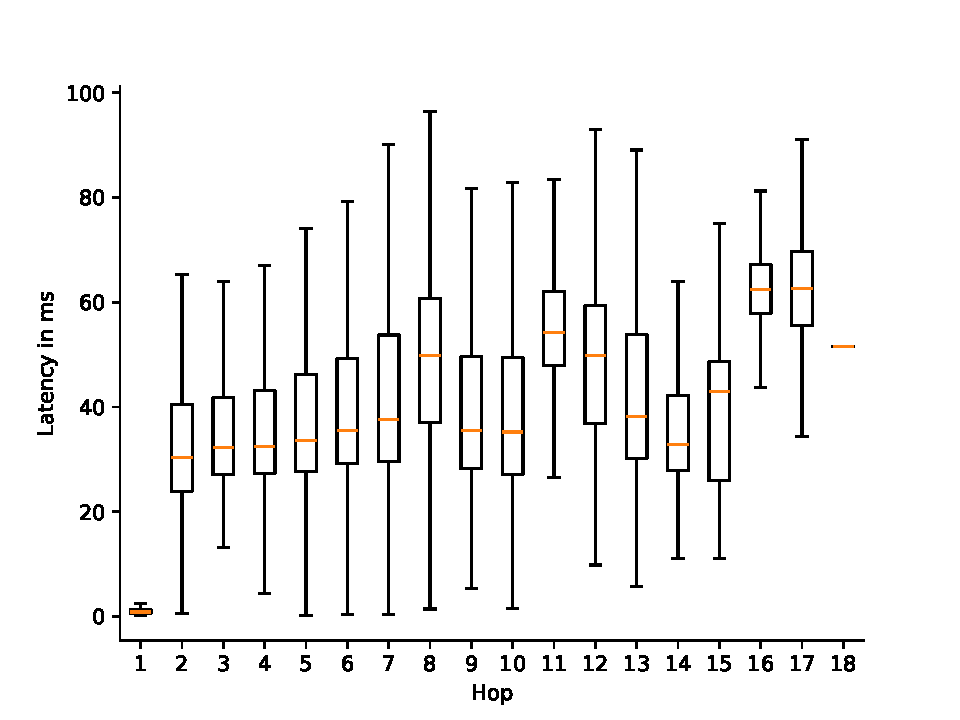
\includegraphics[width=\linewidth]{chapters/4-results/traceroute/img/latency-per-hop-FR.pdf}
		\caption{France}
	\end{subfigure}
	\begin{subfigure}[b]{0.48\linewidth}
		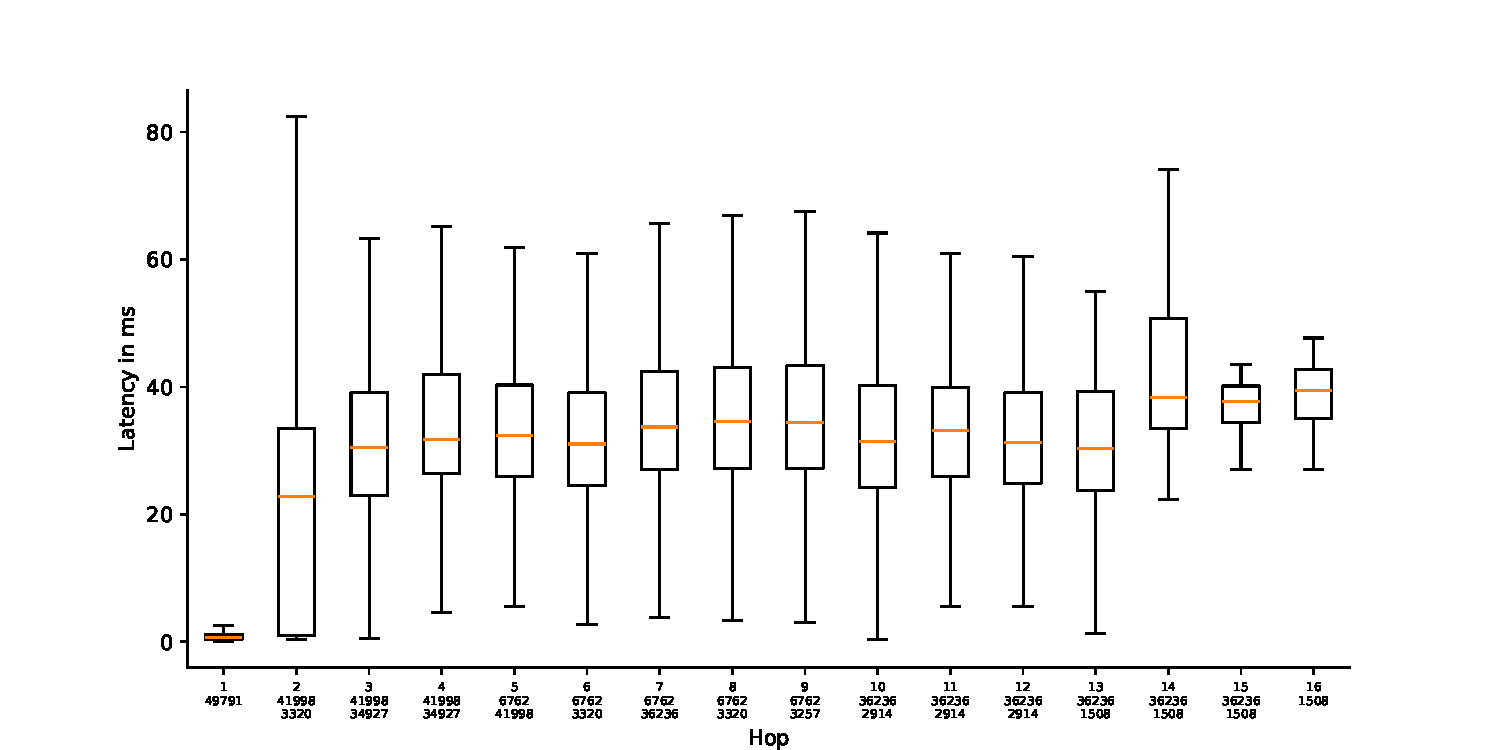
\includegraphics[width=\linewidth]{chapters/4-results/traceroute/img/latency-per-hop-DE.pdf}
		\caption{Germany}
	\end{subfigure}
	\caption{Average Latency per Hop}
	\label{fig:latency-change-per-hop}
\end{figure}

One can see that overall each hop increases the RTT slightly, but in most cases
there is a hop that strongly increases the RTT. We assume that this usually is
the hop from the entry into the satellite constellation toward the \ac{GS}. It
is not clear why this step often appears in a later hop, as the entry into the
satellite constellation should appear as first or second hop.

Also, it is important to note that the behavior is different from country to
country. The appendix shows further countries in
Figure~\ref{fig:latency-change-per-hop-appendix}.
